\subsection{Dense Object Nets}
We implemented training and benchmarking using ``PyTorch-Lightning''\cite{falcon2019pytorch} and ``PyTorch''\cite{paszke2019pytorch} libraries.
Furthermore, we employ
ADAM\cite{kingma2014adam} optimizer to optimize the model for 2500 epochs with a learning rate of
$\alpha = 3 \times 10^{-4}, \beta_1 = 0.9 \text{ and } \beta_2 = 0.999$ with weight decay $\eta =10^{-4}$ to benchmark the DON with Pixelwise NT-Xent loss as in ~\cite{adrian2022efficient}
with a fixed batch size of 1 and 128 image-pair correspondences.
As per the benchmarking results in Table~\ref{table:don_training_results}, the descriptor's robustness increases as the descriptor's dimension gets longer.

\begin{table}[htb]
    \caption{Benchmark of DON framework for GPU consumption and $AUC \pm \sigma$ for $PCK@k,  \forall k \in [1, 100]$ metric.}
    \label{table:don_training_results}
    \centering
    \begin{tabular}{lllll}
        \toprule
        \multicolumn{5}{c}{DON benchmark}                                                                     \\
        \midrule
        Descriptor Size ($D$) & $3 $              & $8 $              & $4 $              & $32$              \\
        AUC for $PCK@k$       & $0.922 \pm 0.006$ & $0.933 \pm 0.011$ & $0.948 \pm 0.012$ & $0.953 \pm 0.008$ \\
        VRAM Usage (GB)       & $9.377 $          & $13.717 $         & $20.479 $         & $30.067$          \\
        \bottomrule
    \end{tabular}
\end{table}

The $AUC \pm \sigma$ for $PCK@k, \forall k \in [1, 100]$ is computed with 256 image-pair correspondences and
the metrics mean and std. deviation is calculated from benchmarking 3 DON models trained for a single descriptor dimension.
We could not train the descriptor dimension of 64 and 128 due to the limited VRAM. Furthermore, to inspect the
results of trained DON, an interface is built using the PyGame library~\cite{pygame} to visualize the results of the trained DON.
The mouse pointer in the image space is mapped to the pixel, and the descriptor at that pixel is queried in another image-descriptor space.
We further use the spatial probability of the descriptor to visualize the queried descriptor
in the image space using Equation~\ref{eqn:gaussian_kernel}
Identify if there are any multi-modal spatial activations in the descriptor spaces and none, as shown in Figure~\ref{fig:check_don}.

\begin{figure}[htb]
    \centering
    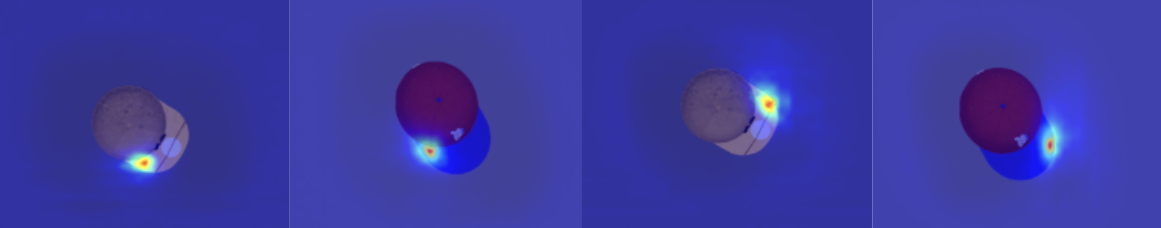
\includegraphics[scale=0.25]{images/test_don.png}
    \caption{Depiction of the spatial probability heatmaps of the descriptor in the image space. We set the temperature in the Equation~\ref{eqn:gaussian_kernel} to $1.1$
        and render the spatial probability heatmaps in the interface. The first and second image from the left and the right highlights the semantically equivalent descriptors in the image space.}
    \label{fig:check_don}
\end{figure}


\subsection{Our Framework}

To train our framework, we employ an ADAM optimizer to optimize the model for 2500 epochs with a learning rate of
$\alpha = 1 \times 10^{-3}, \beta_1 = 0.9 \text{ and } \beta_2 = 0.999$ with no weight decay.
We further use a fixed batch size of 1 and the StepLR scheduler with a step size 2500 and a gamma of 0.9 to train the model with all the loss weights to $1.0$ except variance loss weight to $1 \times 10^{-3}$.
At first, we trained our model with 16 keypoints with a margin of 10 pixels as a hyperparameter for the separation loss, and later, we trained the models with 128 keypoints with a margin of 2 pixels.

\begin{table}[htb]
    \caption{Benchmark of our framework for GPU consumption and $AUC \pm \sigma$ for $PCK@k,  \forall k \in [1, 100]$ metric.}
    \label{table:framework_training_results}
    \centering
    \begin{tabular}{lllll}
        \toprule
        \multicolumn{5}{c}{Our framework with 16 keypoints}                                                          \\
        \midrule
        Descriptor Size ($D$)        & $64 $             & $128 $            & $256 $            & $512$             \\
        $AUC \pm \sigma$ for $PCK@k$ & $0.922 \pm 0.006$ & $0.933 \pm 0.011$ & $0.948 \pm 0.012$ & $0.953 \pm 0.008$ \\
        VRAM Usage (GB)              & $3.799 $          & $4.191 $          & $5.241 $          & $7.341$           \\ \hline
        \multicolumn{5}{c}{Our framework with 128 keypoints}                                                         \\
        \midrule
        Descriptor Size ($D$)        & $64 $             & $128 $            & $256 $            & $512$             \\
        $AUC \pm \sigma$ for $PCK@k$ & $0.922 \pm 0.006$ & $0.933 \pm 0.011$ & $0.948 \pm 0.012$ & $0.953 \pm 0.008$ \\
        VRAM Usage (GB)              & $4.913 $          & $5.409 $          & $6.551$           & $7.915$           \\
        \bottomrule
    \end{tabular}
\end{table}


\subsection{Robot Grasping Pipeline}

For the robot grasping pipeline, we trained our framework with actual caps.
As the synthetic data generation only needs mask and depth information, we could create a mask in no time.
Additionally, while training the framework, we do not need the actual real-world depth information as it computes its own.
We later extracted the dense visual local descriptors from the framework.
We visually inspected for any inconsistencies in the descriptor space, as shown in Figure~\ref{fig:check_real_caps},
and found it consistent. Furthermore, we did not use the models trained on the synthetic dataset, as the representations were inconsistent with the real caps.

\begin{figure}[htb]
    \centering
    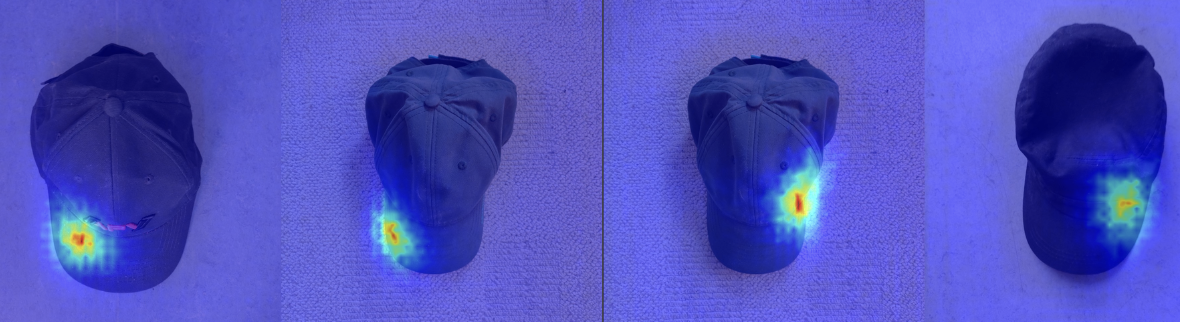
\includegraphics[scale=0.15]{images/test_real_caps.png}
    \caption{Visual inspection of the dense visual descriptors space of the real caps.}
    \label{fig:check_real_caps}
\end{figure}

For robot grasping, a descriptor is picked from the descriptor space and queried in real-time such that robot can pinch-grasp the object.
We could successfully grasp the caps with the robot, as shown in Figure~\ref{fig:straight_grasp}.

\begin{figure}[htb]
    \centering
    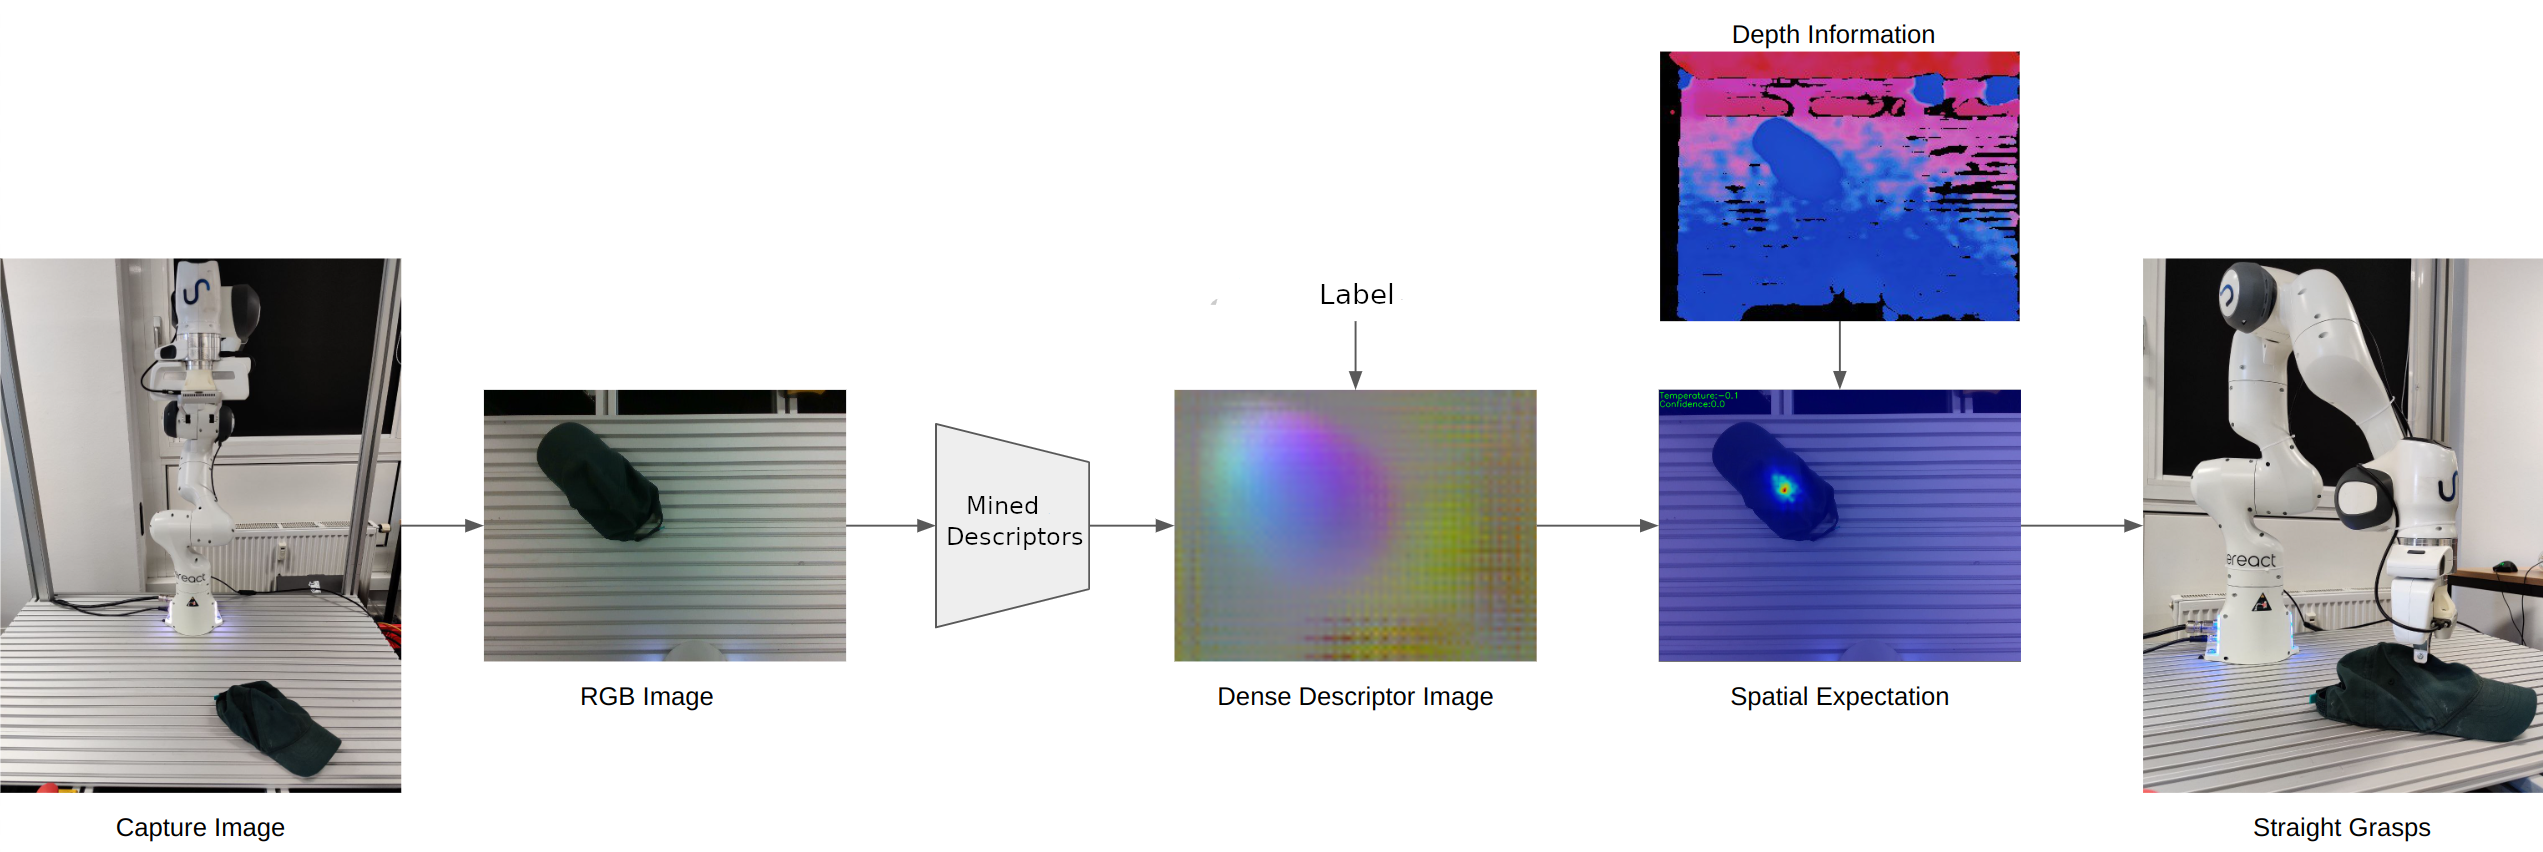
\includegraphics[scale=0.15]{images/straight_grasps.png}
    \caption{Depiction of the straight robot grasping pipeline.}
    \label{fig:straight_grasp}
\end{figure}

As our framework inertly regresses keypoints on the object, we could use it as an alternative approach to grasp the caps by computing the pose
generated by the keypoints considering the actual depth information instead of network-regressed depth information.
We extract the spatial probability of each keypoint from the framework and deactivate spatial probabilities where the depth information is missing,
as the depth image from the camera is noisy. Furthermore, the spatial expectations of the keypoints are projected to the camera frame
to calculate a 6D pose in the camera frame. The 6D pose is transformed in the robot frame to perform an aligned grasp, as shown in Figure~\ref{fig:aligned_grasp}.

\begin{figure}[htb]
    \centering
    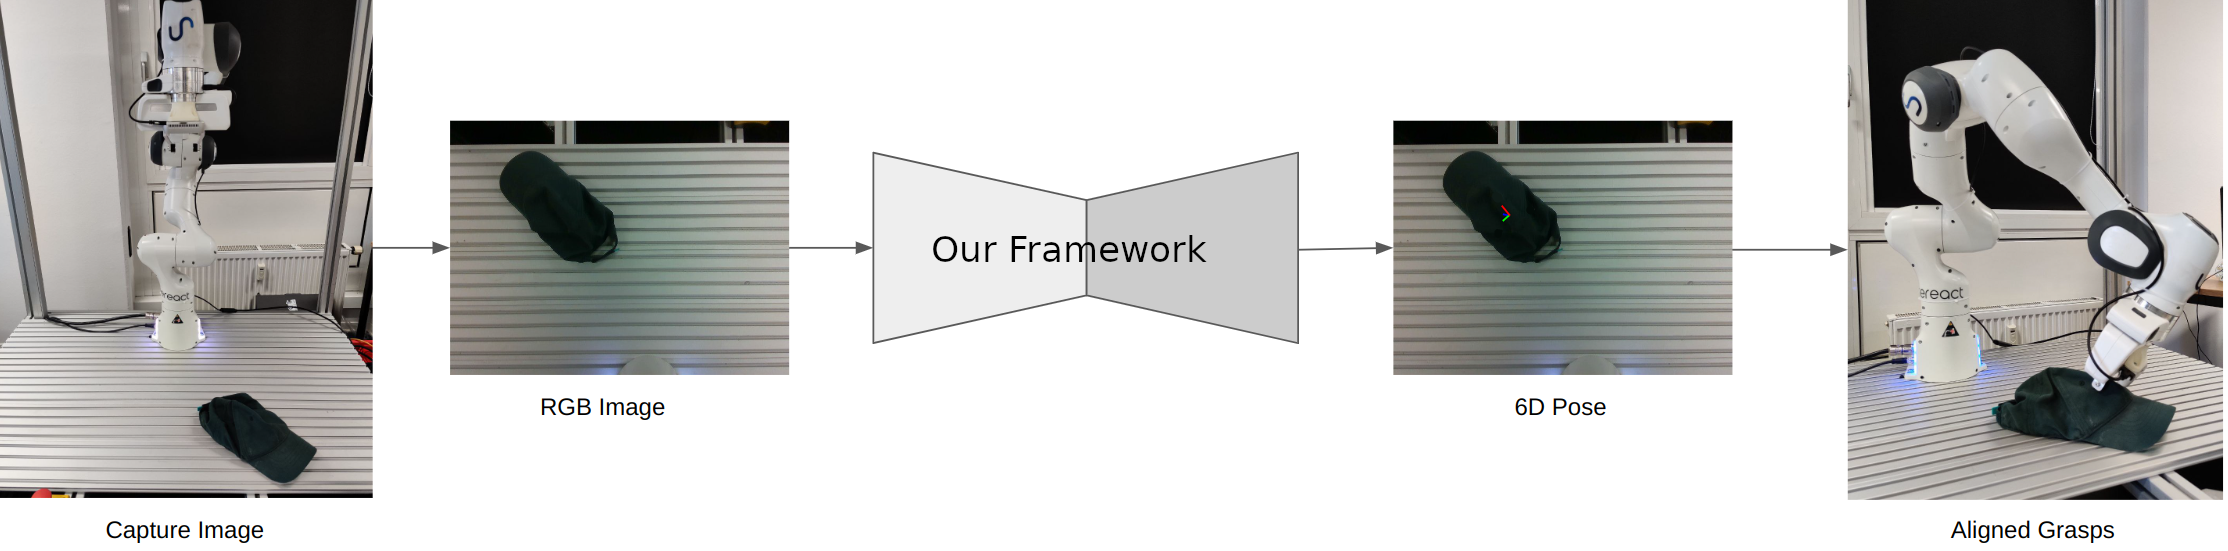
\includegraphics[scale=0.17]{images/aligned.png}
    \caption{Illustration of the aligned robot grasping pipeline.}
    \label{fig:aligned_grasp}
\end{figure}

We did not evaluate the robot grasping pipeline.